%
% ---- PEPA System Models
%

\section{PEPA System Models}\label{sec:pepa-system-models}

The components are combined into models of full distributed architectures, that may be implemented and tested as working built systems.  There are three system models - a simplified microservices architecture, and two models composed of a shared queue and distributed database, with and without replication.

%
% ---- Simple microservices
%
\FloatBarrier
\subsection{Simple microservices}

The simple microservices model has separate end-to-end services for handling athletics and cycling ticket requests.  This is not a `natural' microservices implementation, which would be more likely to separate on operations e.g. searching, booking and returning tickets.  Choosing this design however makes the system directly comparable to the partitioning strategy used for the distributed database models.  It is not in itself functionally different to separating services by operations unless considering additional features to handle eventual data consistency (see Future Work).

The system has two separate databases, one for athletics tickets, one for cycling, and each has its own dedicated worker application (Figure \ref{figure:simplemicro_architecture}).  The PEPA model of this (Figure \ref{figure:simplemicro}) uses the same database process building blocks as the distributed database component models, but in this case they cooperate with the dedicated worker application processes $\mathit{Worker_A}$ and $\mathit{Worker_C}$.

As for the component models, there are two arrival processes, dealing with cycling requests at the rate $\mathit{c=1.0}$ and athletics requests at rates 1.0 to 10.0 in steps of 1.0.  Again each database may serve requests at a maximum rate of {\itshape db}.  Note that this rate has been changed to 6.5 so that it is proportional to the performance observed when testing the built system (the model has been tuned following measurement of the system).

The worker application processes have a maximum rate of $\mathit{w=100.0}$.  This value has been chosen to be much higher than the other parts of the system to minimise its impact on the system testing.  The assumption being made here is that the applications may be designed to cope with this much higher demand, perhaps using Elastic Scaling of servers, which is out of scope of this paper.

\begin{figure}
	\caption{Simple microservices architecture}
	\label{figure:simplemicro_architecture}
	\centering
	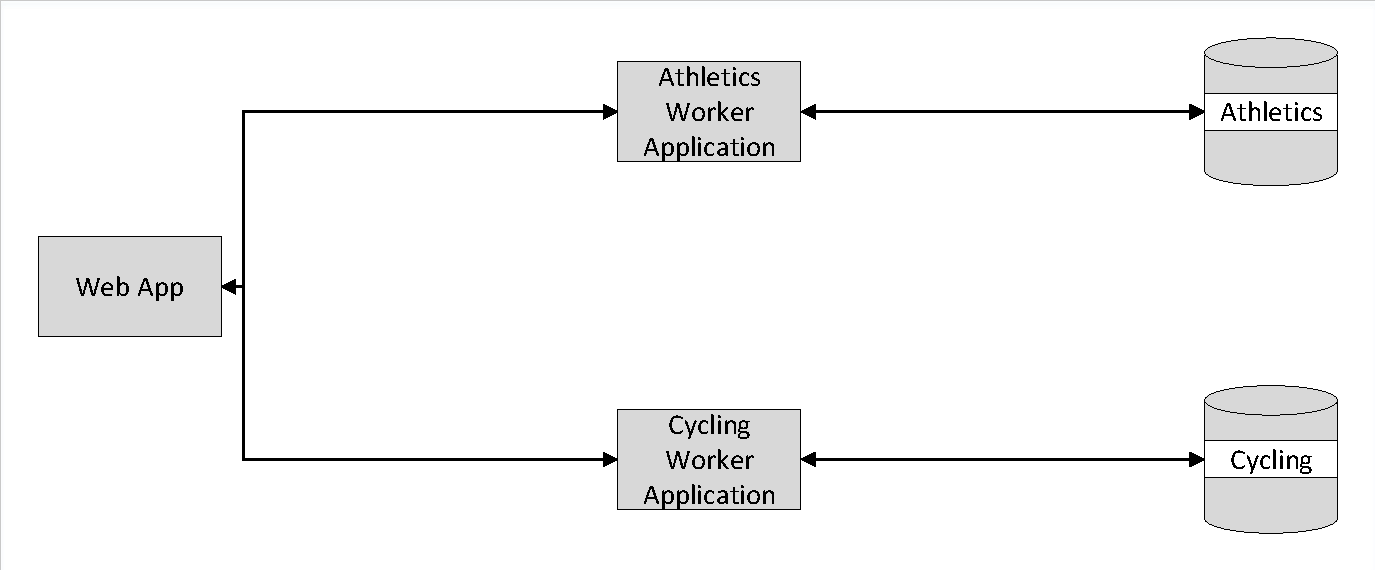
\includegraphics[trim = 5 5 5 5, clip, width=\textwidth]{img/simplemicro}
\end{figure}

\begin{figure}
	\caption{Simple microservices PEPA model}
	\label{figure:simplemicro}
	\centering
	% Automatically generated by PEPA2Latex
	% --begin
	\begin{displaymath}
		\begin{array}{rcl}
			\mathit{a} & = & 1.0 - 10.0\\
			\mathit{c} & = & 1.0\\
			\mathit{w} & = & 100.0\\
			\mathit{db} & = & 6.5\\
			[2.0ex]		\mathit{Website} & \rmdef & (\mathit{athletics},\mathit{a}).\mathit{Website}+(\mathit{cycling},\mathit{c}).\mathit{Website}\\
			\mathit{Worker_A} & \rmdef & (\mathit{athletics},\top).\mathit{WorkerSrv_A}\\
			\mathit{WorkerSrv_A} & \rmdef & (\mathit{workerA},\top).\mathit{Worker_A}\\
			\mathit{Worker_C} & \rmdef & (\mathit{cycling},\top).\mathit{WorkerSrv_C}\\
			\mathit{WorkerSrv_C} & \rmdef & (\mathit{workerC},\top).\mathit{Worker_C}\\
			\mathit{DB_1} & \rmdef & (\mathit{workerA},\mathit{w}).\mathit{DBsrv_1}\\
			\mathit{DBsrv_1} & \rmdef & (\mathit{dbsrv1},\mathit{db}).\mathit{DB_1}\\
			\mathit{DB_2} & \rmdef & (\mathit{workerC},\mathit{w}).\mathit{DBsrv_2}\\
			\mathit{DBsrv_2} & \rmdef & (\mathit{dbsrv2},\mathit{db}).\mathit{DB_2}\\
			\mathit{Service_1} & \rmdef & (\mathit{dbsrv1},\mathit{db}).\mathit{Service_1}\\
			\mathit{Service_2} & \rmdef & (\mathit{dbsrv2},\mathit{db}).\mathit{Service_2}\\
			[2.0ex]		\multicolumn{3}{l}{\mathit{Service_1}\sync{dbsrv1}\mathit{DB_1}\sync{workerA}\mathit{Worker_A}\sync{athletics}\mathit{Website}\sync{cycling}\mathit{Worker_C}\sync{workerC}\mathit{DB_2}\sync{dbsrv2}\mathit{Service_2}}\\
			[2.0ex]	\end{array}
	\end{displaymath}
	% --end
\end{figure}

The PEPA Eclipse plugin experiments test each input rate {\itshape a} of athletics requests from 1.0 to 10.0 in steps of 1.0, with all other rates fixed.  Table \ref{table:micro_results} shows the numerical results, and Figure \ref{figure:micro_charts} shows the throughput of {\itshape athletics} and {\itshape cycling} against input rate {\itshape a}.
These demonstrate that:
\begin{itemize}
	\item the throughput of {\itshape athletics} is constrained by the maximum service rate of the database handling those requests. Both athletics and cycling activities demonstrate some loss of throughput, though less than with the distributed database component (perhaps due to the additional worker application processes producing a partial decoupling effect).
	\item the throughput of {\itshape cycling} is independent of athletics.  This supports the claim that microservices architecture isolates the skewed demand.
	\item the database node throughput follows the throughput of each sport activity.
\end{itemize}

\begin{table}[h!]
	\begin{center}
		\caption{Simple microservices experimental results}
		\label{table:micro_results}
		\pgfplotstabletypeset[
		col sep=comma,
		string type,
		columns/a/.style={column name=a, column type={p{.1\textwidth}}},
		columns/athletics/.style={column name=athletics, column type={p{.1\textwidth}}},
		columns/cycling/.style={column name=cycling, column type={p{.1\textwidth}}},
		columns/workerA/.style={column name=workerA, column type={p{.1\textwidth}}},
		columns/workerC/.style={column name=workerC, column type={p{.1\textwidth}}},
		columns/dbsrv1/.style={column name=dbsrv1, column type={p{.1\textwidth}}},
		columns/dbsrv2/.style={column name=dbsrv2, column type={p{.1\textwidth}}},
		every head row/.style={before row=\hline Rate & \multicolumn{6}{c}{Throughput} \\,after row=\hline},
		every last row/.style={after row=\hline},
		]{data/micro/results.csv}
	\end{center}
\end{table}

\begin{figure}
	\caption{Simple microservices experimental results}
	\label{figure:micro_charts}
	\centering
	\begin{tikzpicture}
	\begin{axis}[
	title={Throughput against input rate a},
	xlabel={Rate a},
	ylabel={Throughput},
	xmin=0, xmax=10,
	ymin=0, ymax=7,
	legend pos=north west,
	ymajorgrids=true,
	grid style=dashed,
	cycle multiindex* list={
		mark list*
		\nextlist
		cyan,brown,green,blue,red
	}
	]
	
	\addplot table [x index={0}, y index={1}, col sep=comma]{data/micro/athletics.csv};
	\addplot table [x index={0}, y index={1}, col sep=comma]{data/micro/cycling.csv};
	
	\legend{athletics,cycling}
	
	\end{axis}
	\end{tikzpicture}
\end{figure}

%
% ---- Shared queue and distributed database
%
\FloatBarrier
\subsection{Shared queue and distributed database}

The next system model (Figure \ref{figure:queuedd_architecture}) is the first combination of the shared queue and distributed database components.  A website sends all ticket requests asynchronously to a cloud queue service, and one or more worker applications (either a multi-threaded application or a scaling set of applications) dequeues the requests and forwards them to the distributed database.  The database uses a horizontal partitioning strategy based on the sport, without any replication.

The PEPA model (Figure \ref{figure:queuedd}) is a straightforward combination of the shared queue and distributed database component models.  A queue length of N=10 is used as the experiments showed that for a small state space, this allowed the athletics throughput to get very close to the maximum service rate.

There is no separate representation of worker processes (the previous system model showed that the throughputs of the worker activities were exactly the same as the processes on either side of them) but as before a high maximum rate has specified $\mathit{q=100.0}$ for the rate at which requests may be dequeued.  This is the rate used for {\itshape queueA} and {\itshape queueB} requests arriving at the database processes.

\begin{figure}
	\caption{Shared queue middleware architecture}
	\label{figure:queuedd_architecture}
	\centering
	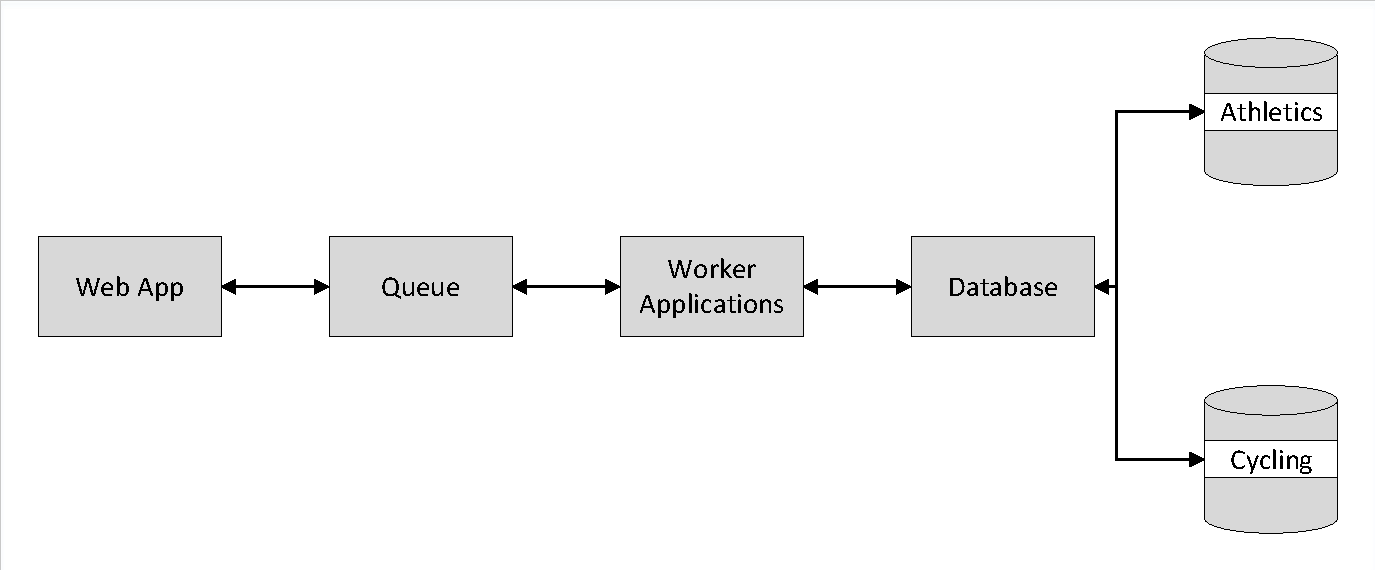
\includegraphics[trim = 5 5 5 5, clip, width=\textwidth]{img/sharedqueue}
\end{figure}

\begin{figure}
	\caption{Shared queue and distributed database}
	\label{figure:queuedd}
	\centering
	% Automatically generated by PEPA2Latex
	% --begin
	\begin{displaymath}
	\begin{array}{rcl}
	\mathit{a} & = & 1.0\\
	\mathit{c} & = & 1.0\\
	\mathit{q} & = & 100.0\\
	\mathit{db} & = & 5.0\\
	[2.0ex]		\mathit{Website} & \rmdef & (\mathit{athletics},\mathit{a}).\mathit{Website}+(\mathit{cycling},\mathit{c}).\mathit{Website}\\
	\mathit{Q_0} & \rmdef & (\mathit{athletics},\top).\mathit{Q_A}+(\mathit{cycling},\top).\mathit{Q_C}\\
	\mathit{Q_A} & \rmdef & (\mathit{queueA},\top).\mathit{Q_0}\\
	\mathit{Q_C} & \rmdef & (\mathit{queueC},\top).\mathit{Q_0}\\
	[2.0ex]		\mathit{DB_1} & \rmdef & (\mathit{queueA},\mathit{q}).\mathit{DBsrv_1}\\
	\mathit{DBsrv_1} & \rmdef & (\mathit{dbsrv1},\mathit{db}).\mathit{DB_1}\\
	\mathit{DB_2} & \rmdef & (\mathit{queueC},\mathit{q}).\mathit{DBsrv_2}\\
	\mathit{DBsrv_2} & \rmdef & (\mathit{dbsrv2},\mathit{db}).\mathit{DB_2}\\
	\mathit{Service_1} & \rmdef & (\mathit{dbsrv1},\mathit{db}).\mathit{Service_1}\\
	\mathit{Service_2} & \rmdef & (\mathit{dbsrv2},\mathit{db}).\mathit{Service_2}\\
	[2.0ex]		\multicolumn{3}{l}{\mathit{Website}\sync{\substack{athletics\\cycling}}\mathit{Q_0}[10]\sync{\substack{queueA\\queueC}}\mathit{DB_1}\parallel\mathit{DB_2}\sync{\substack{dbsrv1\\dbsrv2}}\mathit{Service_1}\parallel\mathit{Service_2}}\\
	[2.0ex]	\end{array}
	\end{displaymath}
	% --end
\end{figure}

As is now usual, the Eclipse plugin is used to find the steady-state throughputs of the activities for input rates of athletics requests increasing from 1.0 to 10.0 with cycling and other rates fixed.  The results appear numerically in Table \ref{table:queuedd_results} and as a chart comparing {\itshape athletics} and {\itshape cycling} throughput in Figure \ref{figure:queueddnr_sport}.
They show:
\begin{itemize}
	\item the throughput of {\itshape athletics} is constrained by the database service rate of a single node.  Athletics and cycling activities demonstrate loss of throughput, but less than shown for the distributed database component alone.  This may indicate the effect of the middleware queue.	
	\item the throughput of {\itshape cycling} is constrained by the ratio between the input rates of athletics and cycling, as it was with the shared queue component.  The behaviour of the queue appears to be the most significant when combined into a system.
	\item the database node throughput follows the throughput of each sport activity, i.e. the partitioning strategy routes all the demand onto the node handling that sport.
\end{itemize}

\begin{table}[h!]
	\begin{center}
		\caption{Shared queue and distributed database experimental results}
		\label{table:queuedd_results}
		\pgfplotstabletypeset[
		col sep=comma,
		string type,
		columns/a/.style={column name=a, column type={p{.1\textwidth}}},
		columns/athletics/.style={column name=athletics, column type={p{.1\textwidth}}},
		columns/cycling/.style={column name=cycling, column type={p{.1\textwidth}}},
		columns/ratio/.style={column name=ratio, column type={p{.1\textwidth}}},
		columns/qa/.style={column name=queueA, column type={p{.1\textwidth}}},
		columns/qc/.style={column name=queueC, column type={p{.1\textwidth}}},
		columns/dbsrv1/.style={column name=dbsrv1, column type={p{.1\textwidth}}},
		columns/dbsrv2/.style={column name=dbsrv2, column type={p{.1\textwidth}}},
		every head row/.style={before row=\hline Rate & \multicolumn{7}{c}{Throughput} \\,after row=\hline},
		every last row/.style={after row=\hline},
		]{data/qddnr/results.csv}
	\end{center}
\end{table}

\begin{figure}
	\caption{Shared queue and distributed database - sport throughput}
	\label{figure:queueddnr_sport}
	\centering
	\begin{tikzpicture}
	\begin{axis}[
	title={Throughput against input rate a},
	xlabel={Rate a},
	ylabel={Throughput},
	xmin=0, xmax=10,
	ymin=0, ymax=5,
	legend pos=north west,
	ymajorgrids=true,
	grid style=dashed,
	cycle multiindex* list={
		mark list*
		\nextlist
		cyan,brown,green,blue,red
	}
	]
	
	\addplot table [x index={0}, y index={1}, col sep=comma]{data/qddnr/athletics.csv};
	\addplot table [x index={0}, y index={1}, col sep=comma]{data/qddnr/cycling.csv};
	
	\legend{athletics,cycling}
	
	\end{axis}
	\end{tikzpicture}
\end{figure}

%
% ---- Shared queue and distributed database with replication
%
\FloatBarrier
\subsection{Shared queue and distributed database with replication}

The final system model (Figure \ref{figure:queueddrep_architecture}) combines a shared queue with a distributed database using replication, with one replica of each data partition on the `next' node using consistent hashing.  As before the website sends ticket requests via a shared queue to a worker application, which dequeues them for the database.

The PEPA model (Figure \ref{figure:queueddrep}) combines the shared queue and distributed database with replication components, so that there is now an additional queue state $\mathit{Q_D}$ for holding {\itshape diving} ticket requests, and there are three data node processes.  $\mathit{DB_1}$ is able to service {\itshape athletics} and {\itshape cycling} requests,  $\mathit{DB_2}$ handles {\itshape cycling} and {\itshape diving}, and $\mathit{DB_3}$ handles {\itshape athletics} and {\itshape diving}.  As with the component node, the model's assumption is that each data node handles each supported sport with equal probability.  Again the model uses a queue length of N=10 and maximum queue worker rate of $\mathit{q=100.0}$.

\begin{figure}
	\caption{Distributed database with replication architecture}
	\label{figure:queueddrep_architecture}
	\centering
	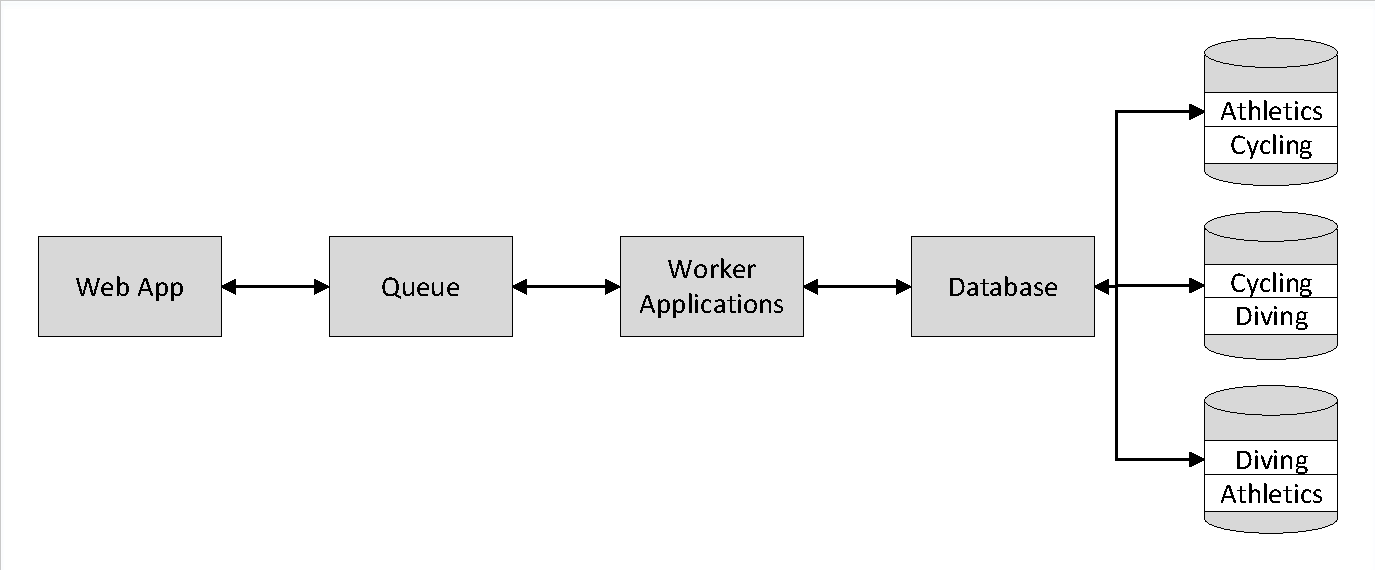
\includegraphics[trim = 5 5 5 5, clip, width=\textwidth]{img/sharedqueue_withrep}
\end{figure}

\begin{figure}
	\caption{Shared queue and distributed database with replication}
	\label{figure:queueddrep}
	\centering
	% Automatically generated by PEPA2Latex
	% --begin
	\begin{displaymath}
	\begin{array}{rcl}
	\mathit{a} & = & 1.0\\
	\mathit{c} & = & 1.0\\
	\mathit{d} & = & 1.0\\
	\mathit{q} & = & 100.0\\
	\mathit{db} & = & 5.0\\
	[2.0ex]		\mathit{Website} & \rmdef & (\mathit{athletics},\mathit{a}).\mathit{Website}+(\mathit{cycling},\mathit{c}).\mathit{Website}+(\mathit{diving},\mathit{d}).\mathit{Website}\\
	\mathit{Q_0} & \rmdef & (\mathit{athletics},\top).\mathit{Q_A}+(\mathit{cycling},\top).\mathit{Q_C}+(\mathit{diving},\top).\mathit{Q_D}\\
	\mathit{Q_A} & \rmdef & (\mathit{queueA},\top).\mathit{Q_0}\\
	\mathit{Q_C} & \rmdef & (\mathit{queueC},\top).\mathit{Q_0}\\
	\mathit{Q_D} & \rmdef & (\mathit{queueD},\top).\mathit{Q_0}\\
	[2.0ex]		\mathit{DB_1} & \rmdef & (\mathit{queueA},\mathit{q}).\mathit{DBsrv_1}+(\mathit{queueC},\mathit{q}).\mathit{DBsrv_1}\\
	\mathit{DBsrv_1} & \rmdef & (\mathit{dbsrv1},\top).\mathit{DB_1}\\
	\mathit{DB_2} & \rmdef & (\mathit{queueC},\mathit{q}).\mathit{DBsrv_2}+(\mathit{queueD},\mathit{q}).\mathit{DBsrv_2}\\
	\mathit{DBsrv_2} & \rmdef & (\mathit{dbsrv2},\top).\mathit{DB_2}\\
	\mathit{DB_3} & \rmdef & (\mathit{queueD},\mathit{q}).\mathit{DBsrv_3}+(\mathit{queueA},\mathit{q}).\mathit{DBsrv_3}\\
	\mathit{DBsrv_3} & \rmdef & (\mathit{dbsrv3},\top).\mathit{DB_3}\\
	\mathit{Service_1} & \rmdef & (\mathit{dbsrv1},\mathit{db}).\mathit{Service_1}\\
	\mathit{Service_2} & \rmdef & (\mathit{dbsrv2},\mathit{db}).\mathit{Service_2}\\
	\mathit{Service_3} & \rmdef & (\mathit{dbsrv3},\mathit{db}).\mathit{Service_3}\\
	[2.0ex]		\multicolumn{3}{l}{\mathit{Website}\sync{\substack{athletics\\cycling\\diving}}\mathit{Q_0}[10]\sync{\substack{queueA\\queueC\\queueD}}\mathit{DB_1}\parallel\mathit{DB_2}\parallel\mathit{DB_3}\sync{\substack{dbsrv1\\dbsrv2\\dbsrv3}}\mathit{Service_1}\parallel\mathit{Service_2}\parallel\mathit{Service_3}}\\
	[2.0ex]	\end{array}
	\end{displaymath}
	% --end
\end{figure}

\FloatBarrier
Experiments are performed in the Eclipse plugin with the usual input rates.  The resulting steady state throughputs are shown in Table \ref{table:queueddwr_results}, in Figure \ref{figure:queueddwr_sport} as a chart comparing {\itshape athletics} and {\itshape cycling} throughput (as the cycling and diving throughputs are identical), and in Figure \ref{figure:queueddwr_database} showing the throughput of the database nodes.
They show:
\begin{itemize}
	\item the throughput of {\itshape athletics} is still constrained but is greater than that of a single database node.  The demand is shared between both data nodes supporting athletics requests.
	\item the throughput of {\itshape cycling} (and diving) is constrained by the ratio between the input rates of athletics and cycling.  In the component model, {\itshape cycling} and {\itshape diving} were impacted by athletics as they both shared a node with athletics tickets.  In the system model, the queue effect appears to outweigh this.
	\item the database node throughput of the two nodes supporting athletics requests is equal, and both are higher than the remaining data node that supports only cycling and diving.  The throughput of this node increases with athletics throughput up to a point, suggesting the node is handling an increasing proportion of the demand for cycling and diving tickets (but that this demand becomes constrained by the queue effect).
	
\end{itemize}

\begin{table}[h!]
	\begin{center}
		\caption{Shared queue and distributed database with replication experimental results}
		\label{table:queueddwr_results}
		\pgfplotstabletypeset[
		col sep=comma,
		string type,
		columns/a/.style={column name=a, column type={p{.07\textwidth}}},
		columns/athletics/.style={column name=athletics, column type={p{.1\textwidth}}},
		columns/cycling/.style={column name=cycling, column type={p{.1\textwidth}}},
		columns/diving/.style={column name=diving, column type={p{.1\textwidth}}},
		columns/ratio/.style={column name=ratio, column type={p{.07\textwidth}}},
		columns/qa/.style={column name=queueA, column type={p{.09\textwidth}}},
		columns/qc/.style={column name=queueC, column type={p{.09\textwidth}}},
		columns/qd/.style={column name=queueD, column type={p{.09\textwidth}}},
		columns/dbsrv1/.style={column name=dbsrv1, column type={p{.09\textwidth}}},
		columns/dbsrv2/.style={column name=dbsrv2, column type={p{.09\textwidth}}},
		columns/dbsrv3/.style={column name=dbsrv3, column type={p{.09\textwidth}}},
		every head row/.style={before row=\hline Rate & \multicolumn{10}{c}{Throughput} \\,after row=\hline},
		every last row/.style={after row=\hline},
		]{data/qddwr/results.csv}
	\end{center}
\end{table}

\begin{figure}
	\caption{Shared queue and distributed database with replication - sport throughput}
	\label{figure:queueddwr_sport}
	\centering
	\begin{tikzpicture}
	\begin{axis}[
	title={Throughput against input rate a},
	xlabel={Rate a},
	ylabel={Throughput},
	xmin=0, xmax=10,
	ymin=0, ymax=9,
	legend pos=north west,
	ymajorgrids=true,
	grid style=dashed,
	cycle multiindex* list={
		mark list*
		\nextlist
		cyan,brown,green,blue,red
	}
	]
	
	\addplot table [x index={0}, y index={1}, col sep=comma]{data/qddwr/athletics.csv};
	\addplot table [x index={0}, y index={1}, col sep=comma]{data/qddwr/cycling.csv};
	
	\legend{athletics,cycling}
	
	\end{axis}
	\end{tikzpicture}
\end{figure}

\begin{figure}
	\caption{Shared queue and distributed database with replication - database throughput}
	\label{figure:queueddwr_database}
	\centering
	\begin{tikzpicture}
	\begin{axis}[
	title={Throughput against input rate a},
	width=0.9\textwidth,
	ybar=0pt,
	bar width=.02\textwidth,
	xlabel={Rate a},
	ylabel={Throughput},
	xtick=data,
	ymin=0, ymax=6,
	legend pos=north west,
	ymajorgrids=true,
	grid style=dashed,
	]
	
	\addplot [pattern=north east lines, pattern color=blue] table [x index={0}, y index={1}, col sep=comma]{data/qddwr/dbsrv_1.csv};
	\addplot [fill=green] table [x index={0}, y index={1}, col sep=comma]{data/qddwr/dbsrv_2.csv};
	\addplot [pattern=crosshatch, pattern color=brown] table [x index={0}, y index={1}, col sep=comma]{data/qddwr/dbsrv_3.csv};
	
	\legend{dbsrv1,dbsrv2,dbsrv3}
	
	\end{axis}
	\end{tikzpicture}
\end{figure}

%
% ---- System comparison
%
\FloatBarrier
\subsection{Comparison}

As the experiments on the three system models all used the same range of input rates {\itshape a} and {\itshape c}, and the throughput of {\itshape athletics} and {\itshape cycling} requests was recorded for each system, then their experimental results may be compared with each other. (Caveat: only the distributed database with replication model has the additional {\itshape diving} activity, but its throughput was identical to diving).  The {\itshape db} rate of the simple microservices model as been set back to 5.0, the same as the other models, and the numerical results of each system model test are compared in Table \ref{table:comparison_results}.  If the models prove to be good representations of built systems, then such comparison shows the strengths and weaknesses of particular distributed system architectures and provides information for decision-making in their selection during design.

\begin{table}[h!]
	\begin{center}
		\caption{Comparison of system results}
		\label{table:comparison_results}
		\pgfplotstabletypeset[
		col sep=comma,
		string type,
		columns/a/.style={column name=a, column type={p{.1\textwidth}}},
		columns/amicro/.style={column name=athletics, column type={p{.15\textwidth}}},
		columns/cmicro/.style={column name=cycling, column type={p{.15\textwidth}}},
		columns/aqddnr/.style={column name=athletics, column type={p{.15\textwidth}}},
		columns/cqddnr/.style={column name=cycling, column type={p{.15\textwidth}}},
		columns/aqddwr/.style={column name=athletics, column type={p{.15\textwidth}}},
		columns/cqddwr/.style={column name=cycling, column type={p{.15\textwidth}}},
		every head row/.style={before row=\hline Rate & \multicolumn{2}{l}{Simple Microservices} & \multicolumn{2}{l}{Queue + Distributed DB} & \multicolumn{2}{l}{Queue + DB with Replication} \\,after row=\hline},
		every last row/.style={after row=\hline},
		]{data/compare.csv}
	\end{center}
\end{table}

\paragraph{Athletics Throughput.}  The comparison shows that the actual throughput of the skewed demand for athletics tickets is lowest for the simple microservices system.  Introducing queue middleware to the system gives a throughput much closer to the maximum service rate of a database node.  Using a distributed database with replication has a load sharing effect so that this system comes closest of all to a throughput that meets the demand.

\paragraph{Cycling Throughput.}  In contrast, the cycling throughput is overall higher for the simple microservices system.  At lower levels of athletics demand, the queue-based systems win out, but as the skewed demand increases then it begins to have an impact on the cycling throughput in these systems.  As the microservices architecture isolates cycling from athletics, it remains at a constant rate.